\documentclass{article}

\usepackage[french]{babel}
\usepackage[T1]{fontenc}
\usepackage{moreverb}       % verbatim with tab

\usepackage{wrapfig}
\usepackage{graphicx}
\usepackage{geometry}
\geometry{hmargin=2.5cm}
\usepackage{amsmath}
\usepackage{siunitx}

\usepackage{graphicx}
\usepackage{subcaption}
\usepackage{float}
\usepackage{hyperref}
\usepackage{setspace}
\usepackage{xcolor}
\usepackage{pdfpages}
\usepackage{enumitem}
\usepackage{lscape}

\usepackage{fancyhdr}       % en-têtes
\usepackage{lastpage}       % numéro de dernière page

\title{Microcontrôleurs\bigbreak \bigbreak
    \large Dossier récapitulatif\bigbreak
    \normalsize Programmation d'un générateur de signaux en assembleur sur PIC16F887\bigbreak}
\date{2020 -- 2021}
\author{Laura Binacchi}

\pagestyle{fancy}
\renewcommand\headrulewidth{1pt}
\fancyhead[L]{Laura Binacchi}
\fancyhead[C]{Microcontrôleurs}
\fancyhead[R]{\today}


\begin{document}
    \pagenumbering{gobble}
    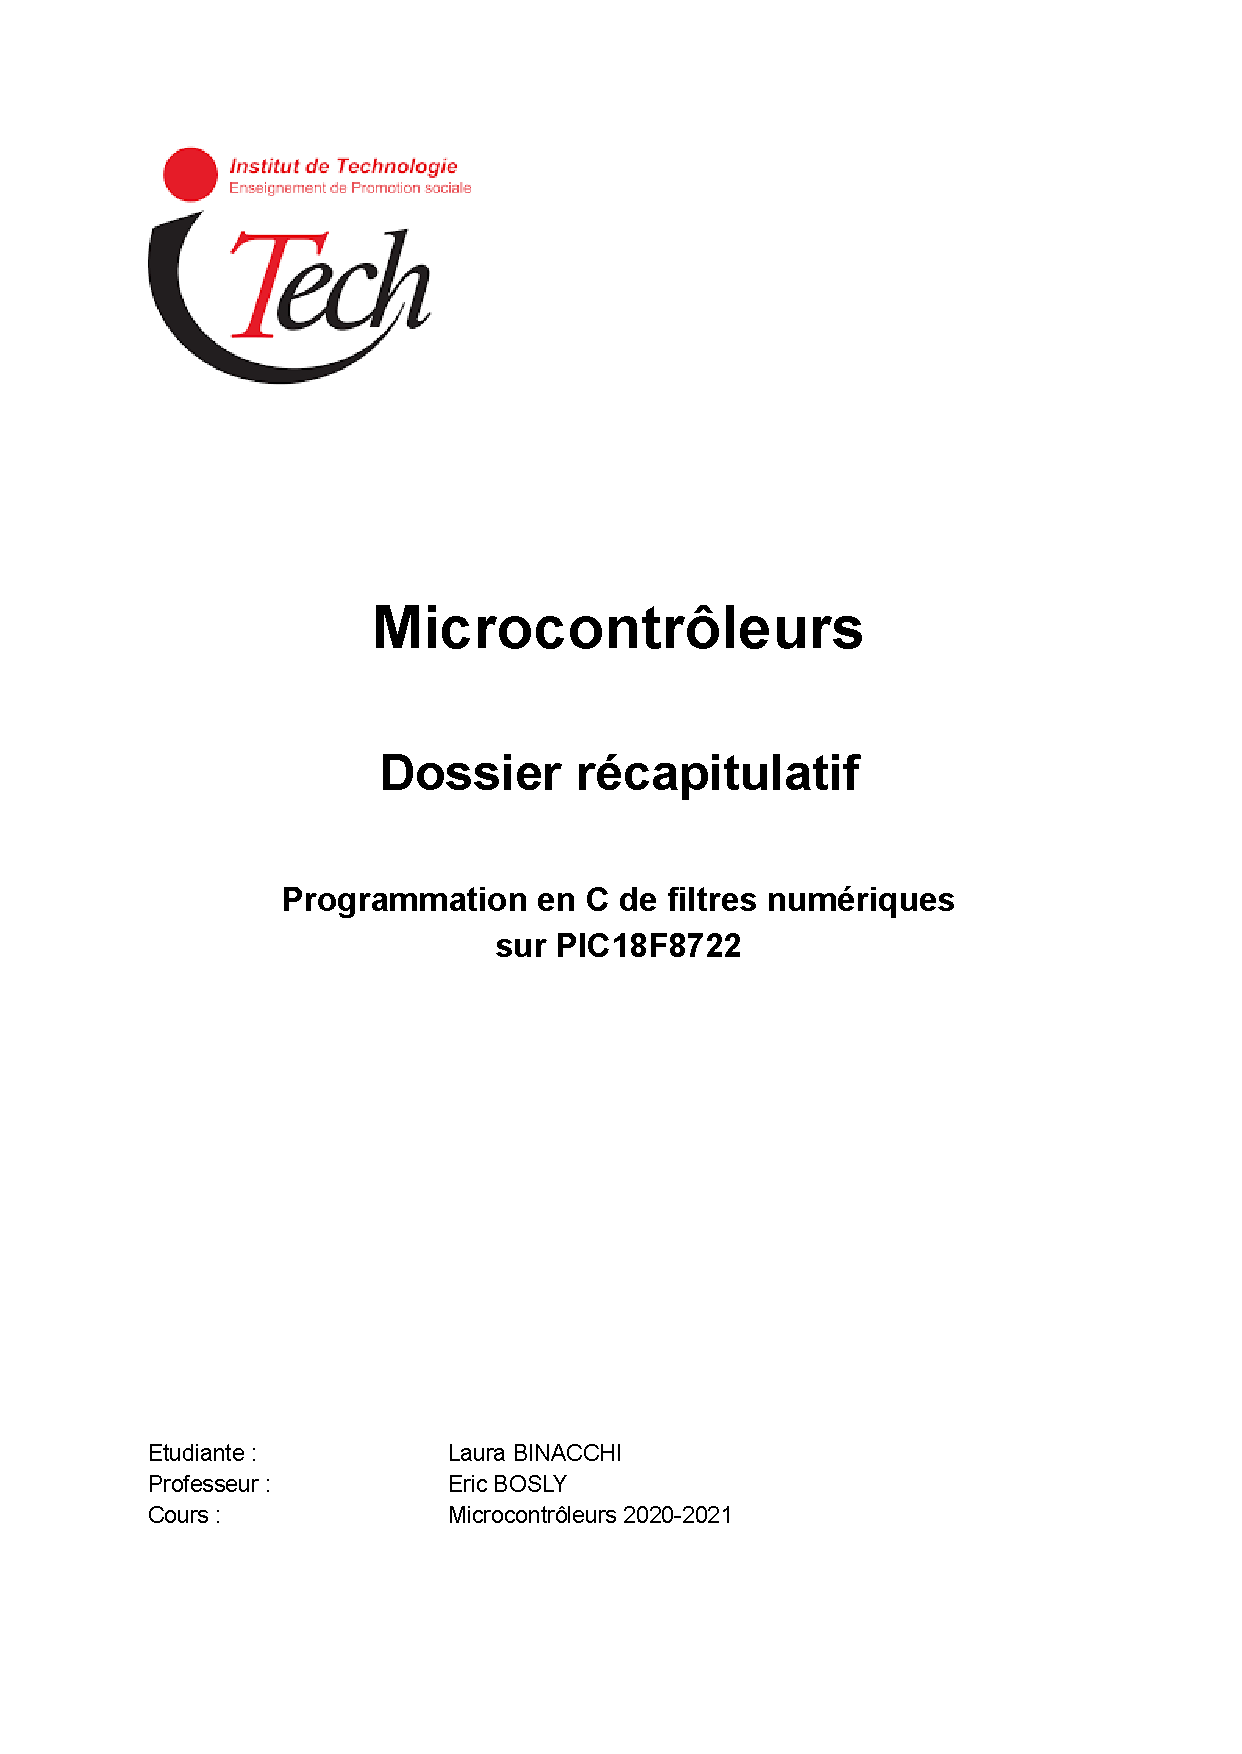
\includepdf[pages={1}]{pdg}
    \newpage
    \tableofcontents
    \newpage
    \pagenumbering{arabic}

    \section{Cahier des charges}

    \subsection{Travail demandé}
    \paragraph{}
    Ecrire un programme en langage C sous MPLABX XC8 pour filtrer un signal sonore mono envoyé à partir d’un fichier .wav sur l’entrée analogique d’un PIC. Ce programme devra tourner sur un PIC18F8722 en simulation Proteus. Ce PIC pilotera un convertisseur NA de sortie permettant d’écouter le résultat des filtres. On respectera les règles de bonne syntaxe vues au cours, notamment en termes de commentaires.

    \paragraph{}
    Un fichier Proteus d’exemple et des fichiers son ont été fournis. L’interface utilisateur du programme est laissée à l’appréciation du développeur, je propose ci-dessous un menu circulaire utilisant le LCD et des boutons poussoirs. Ne perdez cependant pas trop de temps dans ce domaine, ce n’est pas le principal. Le plus important dans ce dossier, sera la mise au point des quatre filtres demandés, programmation et tests.

    \subsection{Cahier des charges de l’application}
    \paragraph{}
    Un signal sonore en mono, généré par une application de type Audacity avec une fréquence d’échantillonnage de 8 ou 16 kHz, est injecté sur une entrée analogique du PIC. Le signal est numérisé sur 8 bits par le module CAN du PIC et filtré en temps réel selon le mode de fonctionnement courant. Le signal filtré est recomposé par un CNA MCP4922 ou DAC0808 au choix, à piloter. Le résultat est audible dans un graphe audio, exportable.

    \paragraph{}
    Connecter un afficheur LCD 4 lignes de 20 caractères, le programme aura plusieurs modes de fonctionnement, résumés dans le tableau ci-dessous.

    \paragraph{}
    La fréquence d’échantillonnage $F_e$ du signal sera configurable à 8kHz ou 16kHz. La fréquence d’échantillonnage conditionne évidement les fréquences de coupure des filtres.

    \paragraph{}
    Le mode « Configuration » et les menus sont laissés à l’appréciation du concepteur. Attention aux conflits potentiels entre le LCD et le convertisseur CNA, si ils utilisent tous les deux une connexion SPI.

    \subsection{Description des 4 filtres demandés}

    \begin{tabular}{l l l}
        Variables           & Y : tampon sortie & X : tampon entrée \\
                            & N : dimension du tampon & \\
                            & A, B : coefficients & \\
                            & & \\
        Moyenne glissante   & $Y_j = \sum\limits_{i=0}^{N-1} \frac{X_{j-i}}{N}$ & pour N = 2 à 8 \\
                            & & \\
        Filtre récursif     & $Y_j = \sum\limits_{i=0}^{N-1} A_i X_{j-i} - \sum\limits_{i=1}^{N-1} B_i X_{j-i}$ & voir fichier tableur joint \\
                            & & \\
        Echo                &  $Y_j = A X_j + B X_{j-del}$ & avec $A + B = 1$ \\
    \end{tabular}

    \paragraph{}
    Le menu décrit ci-dessous est exemplatif, pour éviter de perdre trop de temps avec Proteus, vous pouvez limiter la complexité de l’interface homme-machine.


    \begin{figure}[H]
        \centering
        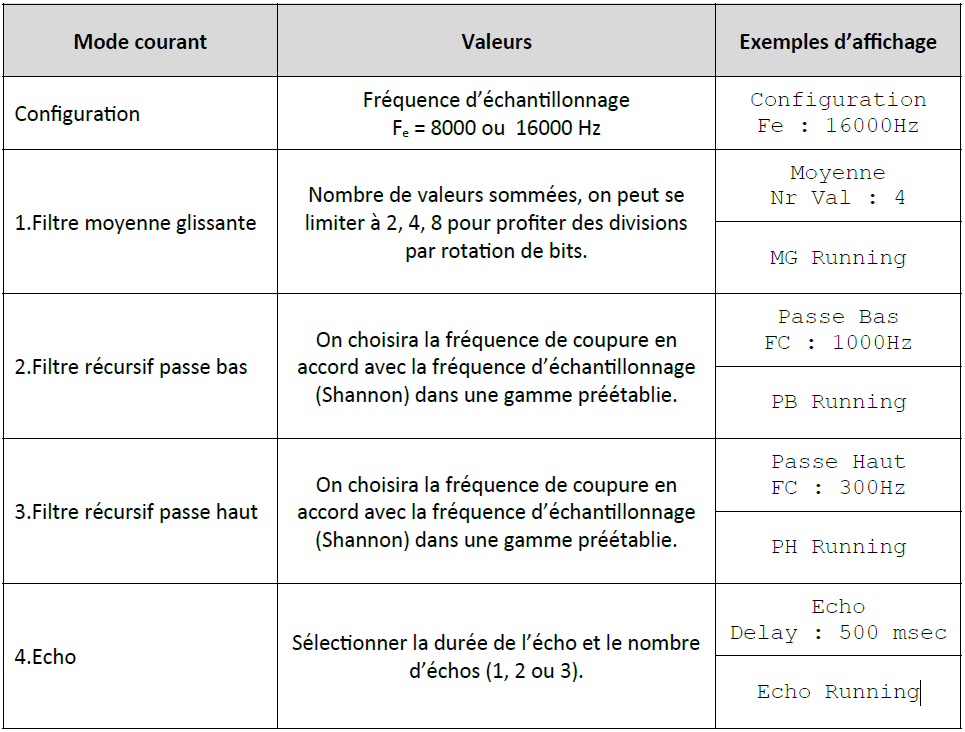
\includegraphics[width=.7\textwidth]{./images/menus.png}
    \end{figure}

    \newpage
    \section{Organigramme de haut niveau}
    \begin{figure}[H]
        \centering
        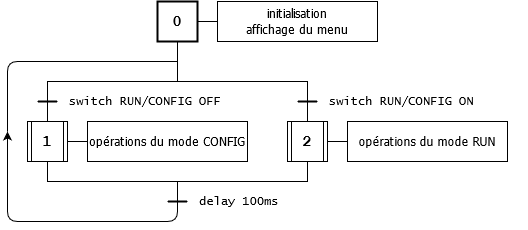
\includegraphics[width=.5\textwidth]{./images/orga_global.png}
        \caption{Organigramme : boucle principale}
    \end{figure}

    \paragraph{}
    Le programme démarre par l'initialisation du PIC \textbf{[0]}. La configuration du PIC et des périphériques (écran LDC et DAC) est détaillée dans la section~\ref{section:configuration}. Les paramètres de traitement du signal et les variables de gestion du menu sont initialisés avec des valeurs par défaut définies pour la plupart (quand cela est possible) par des variables du préprocesseur. Puis le menu est affiché sur l'écran LCD :
    \begin{itemize}
        \item le type de filtre est affiché sur la première ligne;
        \item la fréquence d'échantillonnage est affichée sur la deuxième ligne;
        \item les paramètres du filtre sont affichés sur la troisième et, uniquement dans le cas du filtre echo, sur la quatrième ligne.
    \end{itemize}

    \begin{figure}[H]
        \centering
        \begin{subfigure}[b]{0.34\textwidth}
            \centering
            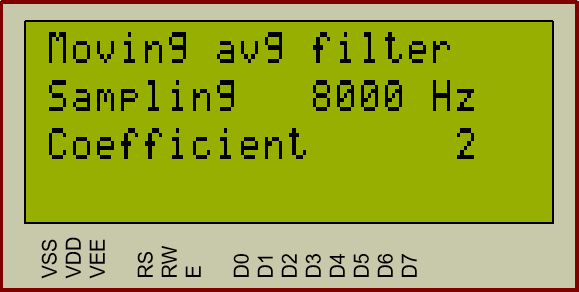
\includegraphics[width=.9\textwidth]{./images/vue_mov_avg.png}
            \caption{Filtre par moyenne glissante}
        \end{subfigure}
        \begin{subfigure}[b]{0.34\textwidth}
            \centering
            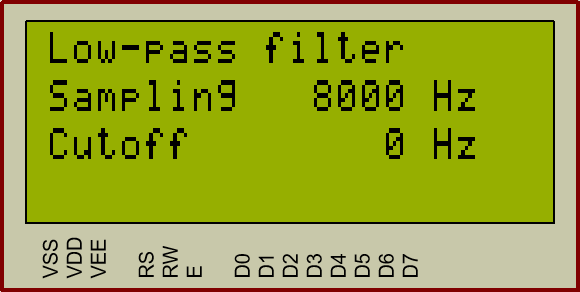
\includegraphics[width=.9\textwidth]{./images/vue_low_pass.png}
            \caption{Filtre passe-bas}
        \end{subfigure}
        \begin{subfigure}[b]{0.34\textwidth}
            \centering
            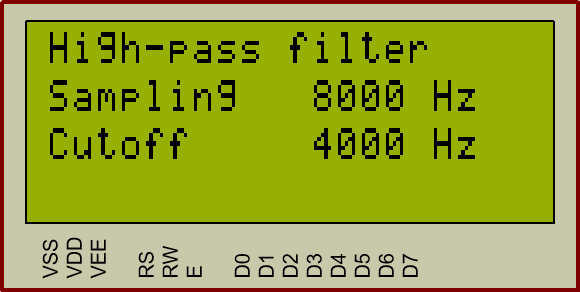
\includegraphics[width=.9\textwidth]{./images/vue_high_pass.png}
            \caption{Filtre passe-haut}
        \end{subfigure}
        \begin{subfigure}[b]{0.34\textwidth}
            \centering
            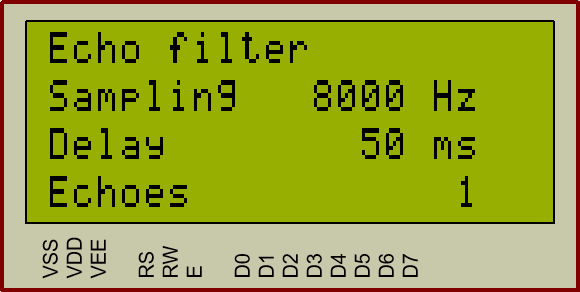
\includegraphics[width=.9\textwidth]{./images/vue_echo.png}
            \caption{Filtre echo}
        \end{subfigure}
        \caption{Vues des différents menus}
   \end{figure}

    \paragraph{}
    En fonction de l'état du switch \texttt{RUN}/$\overline{\texttt{CONFIG}}$, le programme fonctionne soit en mode de configuration \textbf{[1]}, soit en mode de traitement du signal \textbf{[2]}. L'état du switch est scanné en boucle après l'exécution des instructions du mode de fonctionnement sélectionné et une temporisation de \SI{100}{\milli\second}.

    \subsection{Mode de configuration}
    \begin{figure}[H]
        \centering
        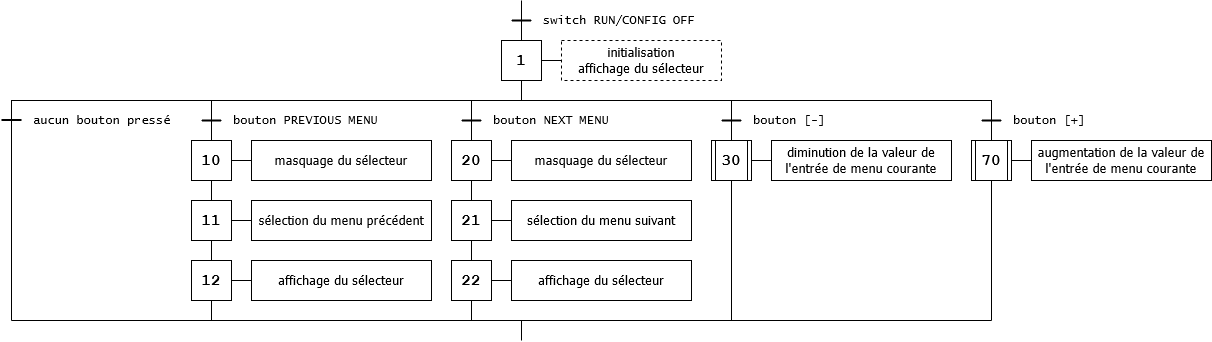
\includegraphics[width=\textwidth]{./images/orga_config.png}
        \caption{Organigramme : mode de configuration}
    \end{figure}

    \paragraph{}
    A son initialisation \textbf{[1]}, le mode de configuration désactive les interruptions de haute priorité, i.e. le traitement du signal, l'entrée de menu active est initialisée au type de filtre et le sélecteur de menu \texttt{<} est affiché sur la ligne correspondante. Grâce à une variable conservant l'état précédant du switch \texttt{RUN}/$\overline{\texttt{CONFIG}}$, le mode de configuration n'est initialisé que lors du passage du mode RUN vers le mode CONFIG.

    \paragraph{}
    Les différents boutons de paramétrage du filtre sont scannés un à un. Si aucun bouton n'est pressé, le programme continue de scanner les entrées tant que le mode de configuration est actif. Si plusieurs boutons sont pressés en même temps, seul le premier est pris en compte selon l'ordre dans lequel ils sont scannés.

    \paragraph{}
    Les boutons \texttt{PREVIOUS} et \texttt{NEXT} permettent de naviguer dans le menu. Lorsque le bouton \texttt{PREVIOUS} est pressé puis relâché, le sélecteur de menu est effacé \textbf{[10]}. L'entrée de menu précédente est sélectionnée \textbf{[11]} en mettant à jour la variable du programme qui garde en mémoire l'entrée de menu courante. Puis le sélecteur est affiché sur la nouvelle entrée active \textbf{[12]}. Si la première entrée du menu est active lorsque le bouton \texttt{PREVIOUS} est pressé, c'est la dernière entrée du menu qui devient active.

    \begin{figure}[H]
        \centering
        \begin{subfigure}[b]{.34\textwidth}
            \centering
            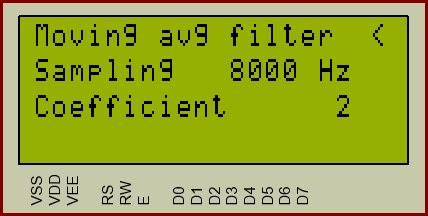
\includegraphics[width=.9\textwidth]{./images/previous_a.png}
        \end{subfigure}
        \begin{subfigure}[b]{.34\textwidth}
            \centering
            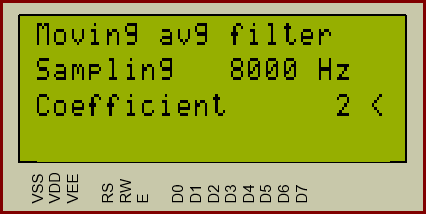
\includegraphics[width=.9\textwidth]{./images/previous_b.png}
        \end{subfigure}
        \caption{Passage du sélecteur de la première à la dernière entrée lorsque le bouton \texttt{PREVIOUS} est pressé}
    \end{figure}

    \paragraph{}
    De la même manière, lorsque le bouton \texttt{NEXT} est pressé puis relâché, le sélecteur de menu est effacé \textbf{[20]}, l'entrée de menu suivante est sélectionnée \textbf{[21]} puis le sélecteur est affiché sur la nouvelle entrée de menu active \textbf{[22]}.

    \paragraph{}
    Les boutons \texttt{[-]} et \texttt{[+]} permettent de modifier le type de filtre et ses paramètres en diminuant \textbf{[30]} ou augmentant \textbf{[70]} la valeur de l'entrée de menu active.

    \begin{figure}[H]
        \centering
        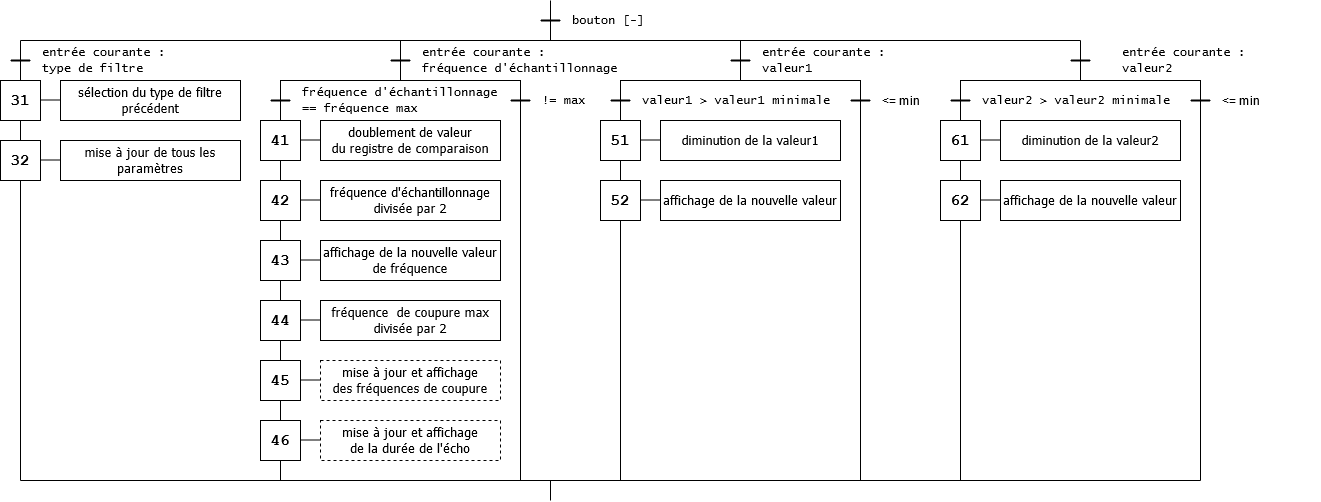
\includegraphics[width=\textwidth]{./images/orga_decrease.png}
        \caption{Organigramme : diminution de la valeur de l'entrée de menu active}
    \end{figure}

    \paragraph{}
    La modification du type de filtre \textbf{[31]} se fait, comme la navigation, de manière circulaire : il tourne en boucle en appuyant sur le bouton \texttt{[+]} ou sur le bouton \texttt{[-]}, dans un sens de défilement ou dans l'autre. Lorsque le type de filtre est modifié, c'est tout l'affichage qui est mis à jour \textbf{[32]} car les paramètres configurables dépendent du type de filtre actif.

    \paragraph{}
    La fréquence d'échantillonnage n'a que deux valeurs possibles : \SI{8}{\kilo\hertz} ou \SI{16}{\kilo\hertz}. Elle n'est donc diminuée que si elle est au maximum (de la même manière, elle ne sera augmentée que si elle est au minimum). La valeur de comparaison de l'interruption est doublée \textbf{[41]} et la valeur de la fréquence d'échantillonnage est divisée par deux \textbf{[42]} puis mise à jour sur le LCD \textbf{[43]}. La fréquence d'échantillonnage détermine la fréquence de coupure maximale qui peut être utilisée par les filtres : ce maximum est fixé à la moitié de la fréquence d'échantillonnage \textbf{[44]} (théorème de Shannon). Si les fréquences de coupure des filtres passe-bas et passe-haut dépassent cette valeur maximale, elles prennent cette nouvelle valeur et, si filtre actif est un filtre passe-bas ou passe-haut, le LCD est mis à jour \textbf{[45]}. La fréquence d'échantillonnage détermine également la valeur maximale que peut prendre la durée de l'écho : lorsque la fréquence est divisée par deux, la durée de l'écho est doublée et si le filtre écho est sélectionné, la nouvelle valeur est affichée \textbf{[46]}.

    \paragraph{}
    La diminution de la première valeur met à jour \textbf{[51]}, en fonction du filtre actif, soit : le coefficient du filtre par moyenne glissante; la fréquence de coupure du filtre passe-bas; la fréquence de coupure du filtre passe-haut; le délai du filtre echo.

    \paragraph{}
    La deuxième valeur \textbf{[61]} ne concerne que le filtre echo et met à jour le nombre d'échos.

    \paragraph{}
    Ces valeurs ne peuvent être diminuées que si elles sont strictement supérieures aux valeurs minimales définies par des variables du préprocesseur. Elles sont diminuées d'un pas également défini par des variables du préprocesseur. Le même mécanisme est implémenté pour l'augmentation des valeurs.

    \subsection{Mode de traitement du signal}
    \begin{figure}[H]
        \centering
        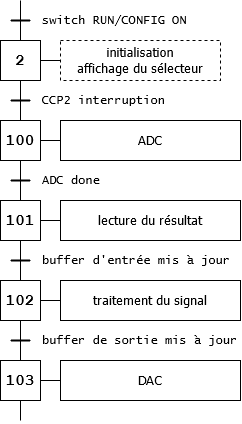
\includegraphics[width=.2\textwidth]{./images/orga_run.png}
        \caption{Organigramme : mode de traitement du signal}
    \end{figure}

    \paragraph{}
    Comme le mode de configuration, le mode de traitement du signal n'est initialisé que lors du passage du mode \texttt{CONFIG} au mode \texttt{RUN} \textbf{[2]} : le sélecteur de menus \texttt{<} est masqué et le signal est initialisé en fonction du type de filtre actif et de ses paramètres.

    \paragraph{}
    Une interruption survient toutes les \SI{125}{\micro\second} (fréquence d'échantillonnage à \SI{8}{\kilo\hertz}) ou toutes les \SI{62,5}{\micro\second} (fréquence d'échantillonnage à \SI{16}{\kilo\hertz}). Elle déclenche la conversion analogique-numérique (ADC) \textbf{[100]}. Quand elle est terminée, son résultat est lu dans le tampon d'entrée \textbf{[101]}. Le signal est alors traité selon le type de filtre et ses paramètres \textbf{[102]} et la résultat du traitement est placé dans le tampon de sortie pour pouvoir être transmis au convertisseur numérique analogique (DAC) \textbf{[103]}.



    \section{Fréquences utilisées}
    \paragraph{}
    Le cahier des charges demande d'implémenter des fréquences d'échantillonnage de 8 et de \SI{16}{\kilo\hertz}. Conformément au théorème de de Nyquist-Shannon les fréquences utiles des signaux sont donc respectivement limitées à 4 et à \SI{8}{\kilo\hertz}.

    \paragraph{}
    Les différents signaux testés ont été échantillonnés à 8 ou à \SI{16}{\kilo\hertz} permettant de se passer d'un filtre anti-repliement à l'entrée du signal. En sortie, les filtres de Laplace sont réglés à la fréquence utile du signal testé.

    \paragraph{}
    Les analyses de Fourier présentent également le spectre de fréquence sur la plage de fréquence utile du signal, soit 8 ou \SI{16}{\kilo\hertz}.

    \paragraph{}
    La fréquence d'échantillonnage est implémentée par le programme en déclenchant une interruption à un intervalle déterminé : toutes les \SI{125}{\micro\second} pour du \SI{8}{\kilo\hertz} ou toutes les \SI{62.5}{\micro\second} pour du \SI{16}{\kilo\hertz}. La configuration de l'interruption est détaillée à la section~\ref{section:interruption}.



    \section{Configuration du PIC}
    \label{section:configuration}

    \paragraph{}
    Le PIC est configuré par les instructions d'initialisation de ses différents registres aux lignes 250 à 270 du fichier \emph{main.c} et par les directives de préprocesseur (\emph{pragmas}) aux lignes 28 à 100.

    \subsection{Oscillateur}
    La première directive de préprocesseur configure l'oscillateur en mode HSPLL. Ce mode multiplie par 4 la fréquence de l'oscillateur. Une fréquence de \SI{10}{\mega\hertz} correspond donc à un temps de cycle CPU de \SI{0.1}{\micro\second}.
    \begin{verbatimtab}
     [29]    #pragma config OSC = HSPLL
    \end{verbatimtab}

    \subsection{Interruption}
    \label{section:interruption}
    \paragraph{}
    Le traitement du signal est effectué par une interruption générée par le module CCP2 et le Timer1. Le module CCP2 est activé en mode comparateur avec special event trigger : à chaque interruption, le timer est réinitialisé et la conversion analogique-digitale est déclenchée automatiquement.
    \begin{verbatimtab}
    [258]    CCP2CON = 0x0B;         // CCP2 interruption in compare mode
                                             with trigger special event
    \end{verbatimtab}

    \paragraph{}
    Le Timer1 est activé avec un prescaler 1:1 : une valeur de comparaison de 1 déclencherait une interruption tous les cycles CPU, i.e. toutes les \SI{0.1}{\micro\second}.
    \begin{verbatimtab}
    [261]    T1CON   = 0x01;         // Timer1 prescale 1:1
    [262]    TMR1H   = 0;            // Timer1 -> 0
    [263]    TMR1L   = 0;
    \end{verbatimtab}

    \paragraph{}
    La valeur de comparaison est initialisée à 1250 (\texttt{0x04E2}). L'interruption surviendra donc toutes les \SI{125}{\micro\second}, ce qui correspond à une fréquence de \SI{8}{\kilo\hertz}. Pour fonctionner à une fréquence d'échantillonnage de \SI{16}{\kilo\hertz}, cette valeur est divisée par 2.
    \begin{verbatimtab}
    [259]    CCPR2H  = 0x04;         // 1250us -> 8kHz
    [260]    CCPR2L  = 0xE2;
    \end{verbatimtab}

    \paragraph{}
    Les interruptions prioritisées sont activées et les interruptions de haute et de basse priorité sont désactivées. Les interruptions de haute priorité seront activée après l'initialisation si le mode de traitement du signal est actif.
    \begin{verbatimtab}
    [264]    RCONbits.IPEN   = 1;    // enable priority levels on interrupts
    [265]    INTCONbits.GIEH = 0;    // high priority interrupts disabled
    [266]    INTCONbits.GIEL = 0;    // low priority interrupts disabled
    \end{verbatimtab}

    \paragraph{}
    Une haute priorité est accordée à l'interruption par le module CCP2. L'interruption est activée (et son flag effacé). Elle ne sera effectivement active que quand les interruptions de haute priorité auront été activées.
    \begin{verbatimtab}
    [267]    IPR2bits.CCP2IP = 1;    // CCP2 interrupt: high priority
    [268]    PIE2bits.CCP2IE = 1;    // CCP2 interrupt enabled
    [269]    PIR2bits.CCP2IF = 0;    // CCP2 interrupt flag cleared
    \end{verbatimtab}

    \subsection{Conversion analogique-digitale}
    \paragraph{}
    La conversion analogique-digitale est activée par le registre \texttt{ADCON0} qui sélectionne également l'entrée analogique au convertisseur : la canal 0. Le registre \texttt{ADCON1} configure la PIN AN0 en analogique (le minimum nécessaire) et garde les tensions de référence par défaut : $A_{VDD}$ et $A_{VSS}$ (0 et \SI{5}{\volt}).
    \begin{verbatimtab}
    [255]    ADCON0  = 0X01;         // ADC enabled on AN0
    [256]    ADCON1  = 0x0E;         // AN0 -> analogic
    [257]    ADCON2  = 0x01;         // Left justification, 0 Tad, Fosc/8
    \end{verbatimtab}

    \paragraph{}
    Le registre \texttt{ADCON2} sélectionne la justification à gauche du résultat de la conversion dans les registres \texttt{ADRESH} et \texttt{ADRESL} : le programme travaille en 8bits et ne conserve donc que les 8 bits de poids forts lus dans le registre \texttt{ADRESH}.

    \paragraph{}
    Le registre \texttt{ADCON2} permet aussi de définir le temps d'acquisition et la fréquence de conversion. Le temps d'acquisition est configuré à 0 $T_{AD}$ car les conversions sont effectuées selon la fréquence des interruptions (maximum à \SI{16}{\kilo\hertz}) : il se sera donc toujours passé assez de temps entre les conversions. La fréquence de conversion est choisie en fonction de la fréquence de l'oscillateur et du type de PIC conformément à la table 21-1 (\emph{TAD vs. DEVICE OPERATING FREQUENCIES}) de la datasheet. Elle est de 8 $T_{OSC}$ pour une fréquence d'oscillateur de \SI{10}{\mega\hertz} en respectant la recommendation de la datasheet de choisir le plus petit temps supérieur au minimum requis.

    \subsection{Bus SPI et périphériques}
    \paragraph{}
    Le bus SPI et les périphériques qui y sont associés sont initialisés par la fonction \texttt{init\_SPI()} du fichier \emph{SPI.c}. Cette fonction est reprise de la librairie de gestion de la communication d'un PIC avec un LCD fournie pour les projets précédents.

    \subsection{I/O}
    \paragraph{}
    Les boutons de gestion du menu sont connectés directement au PORTE du PIC. Le registre TRISE est donc configuré en input.
    \begin{verbatimtab}
    [250]    TRISE   = 0xFF;         // PORTE (menu buttons) -> input
    \end{verbatimtab}

    \paragraph{}
    Le projet aurait pu implémenter une lecture des entrées via le bus SPI et une interruption de faible priorité. Ce n'est pas le cas car le programme principal utilise déjà le bus SPI pour communiquer avec le LCD et les communications entreraient en conflit.

    \paragraph{}
    La PIn permettant de vérifier le temps d'exécution de l'interruption est configurée en output et initialisée à 0.
    \begin{verbatimtab}
    [251]    TRISGbits.TRISG0 = 0;   // TICK -> output
    [252]    TICK    = 0;            // TICK -> 0
    \end{verbatimtab}

    \paragraph{}
    Enfin, bien que le projet permette de générer un signal via le convertisseur digital-analogique MCP4922, le DAC0808 n'a pas été supprimé car tous les tests présentés ont été fait avec ce DAC.
    \begin{verbatimtab}
    [253]    TRISD   = 0;            // DAC0808 -> output
    [254]    DAC0808 = 128;          // DAC0808 -> 0 + offset
    \end{verbatimtab}



    \section{Tests}
    \paragraph{}
    Tout au long du développement, le programme a été testé avec la simulation Proteus et les différents outils à disposition. L'oscilloscope branché sur les différentes PIN a permis de vérifier la génération d'un signal en sortie des DAC et en sortie des filtres de Laplace mais aussi de s'assurer que la durée de traitement ne dépasse pas la durée de l'interruption grâce à la PIN activée durant le traitement du signal ou encore de débugger les communications via le bus SPI.

    \paragraph{}
    Une fois la programmation du filtre terminée, la sortie des filtres a été validée avec les analyses de Fourier et les analyses de signaux audio générées dans Proteus. Ce sont les résultats de ces tests qui sont présentés dans cette section. Ils ont été produits en changeant les paramètre d'initialisation du filtre avant la compilation du programme. Tous les tests réalisés se trouvent dans le code source et il suffit de décommenter le test souhaité pour le reproduire.

    \paragraph{}
    Pour les différents tests, les fréquences de coupures des filtres de Laplace en sortie des DAC on été réglées soit à \SI{8}{\kilo\hertz} soit à \SI{4}{\kilo\hertz} en fonction de la fréquence d'échantillonnage testée (ce paramètre est affiché sous le filtre dans le projet Proteus).

    \paragraph{}
    Tous les signaux utilisés pour les tests et tous les signaux générés par les tests se trouvent dans le dossier \emph{wav} du projet.


    \subsection{Filtre par moyenne glissante}
    \paragraph{}
    Les tests du filtre par moyenne glissante ont été effectués sur l'audio \emph{drake\_30s\_delay\_1s\_8k.wav} pour les tests faits avec une fréquence d'échantillonnage de \SI{8}{\kilo\hertz} et \emph{drake\_30s\_delay\_1s\_16k.wav} pour une fréquence d'échantillonnage de \SI{16}{\kilo\hertz}. Le délai d'une seconde permet de laisser le temps au programme de s'initialiser.

    \paragraph{}
    Le filtre par moyenne glissante implémente assez peu de combinaisons possibles de coefficient et de fréquence d'échantillonnage que pour pouvoir les tester toutes.

    \paragraph{}
    Que ce soit en \SI{16}{\kilo\hertz} ou en \SI{8}{\kilo\hertz}, les tests mettent en évidence que le filtre est d'autant plus filtrant que son coefficient est élevé. Plus le coefficient augmente, plus le signal de sortie est atténué par rapport au signal d'entrée. Les fréquences du signal de sortie sont également de plus affaiblies à mesure que le coefficient du filtre augmente.

    \paragraph{}
    Les hautes fréquences sont par contre plus puissantes pour le signal de sortie que pour le signal d'entrée : il s'agit du bruit de quantification. Ce bruit n'est pas lié au filtre mais au traitement numérique d'un signal analogique : il apparaît également quand le signal lu est directement reporté sur la DAC.

    \begin{figure}[H]
        \centering
        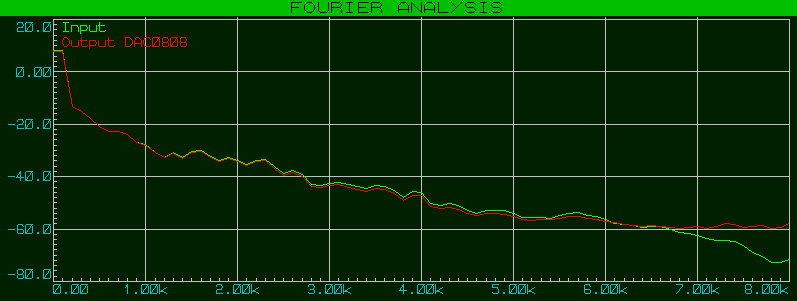
\includegraphics[width=.6\textwidth]{./images/spectrum_no_filter_drake_16k.png}
        \caption{Spectre des signaux d'entrée et de sortie, pas de filtre (16kHz)}
    \end{figure}

    \paragraph{}
    Les fichiers audio produits permettent également d'entendre la dégradation progressive du signal : à mesure que le coefficient du filtre augmente, le son paraît de plus en plus étouffé. Les signaux produits sont enregistrés dans les fichiers :
    \begin{itemize}
        \item \emph{test\_mov\_avg\_2\_16k.wav} (filtre d'ordre 2 en \SI{16}{\kilo\hertz})
        \item \emph{test\_mov\_avg\_4\_16k.wav} (filtre d'ordre 4 en \SI{16}{\kilo\hertz})
        \item \emph{test\_mov\_avg\_8\_16k.wav} (filtre d'ordre 8 en \SI{16}{\kilo\hertz})
        \item \emph{test\_mov\_avg\_2\_8k.wav} (filtre d'ordre 2 en \SI{8}{\kilo\hertz})
        \item \emph{test\_mov\_avg\_4\_8k.wav} (filtre d'ordre 4 en \SI{8}{\kilo\hertz})
        \item \emph{test\_mov\_avg\_8\_8k.wav} (filtre d'ordre 8 en \SI{8}{\kilo\hertz})
    \end{itemize}

    \paragraph{}
    Dans tous les tests, le signal de sortie apparaît légèrement déphasé par rapport au signal d'entrée. Cet effet est principalement dû au filtre de Laplace plus qu'au temps de traitement du signal.

    \begin{figure}[H]
        \centering
        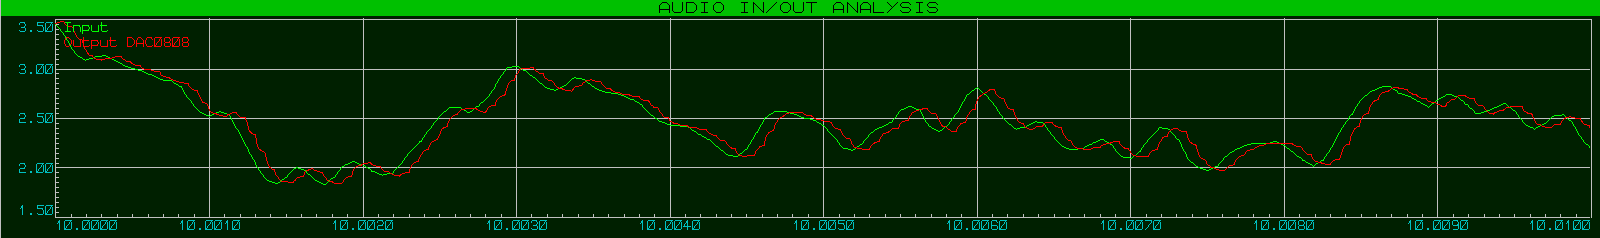
\includegraphics[width=\textwidth]{./images/out_no_filter_drake_16k.png}
        \caption{Signal de sortie déphasé par rapport au signal d'entrée, pas de filtre (16kHz)}
    \end{figure}

%     \subsubsection{Test : filtre d'ordre 2 (16kHz)}
%     \begin{figure}[H]
%         \centering
%         \begin{subfigure}[b]{\textwidth}
%             \centering
%             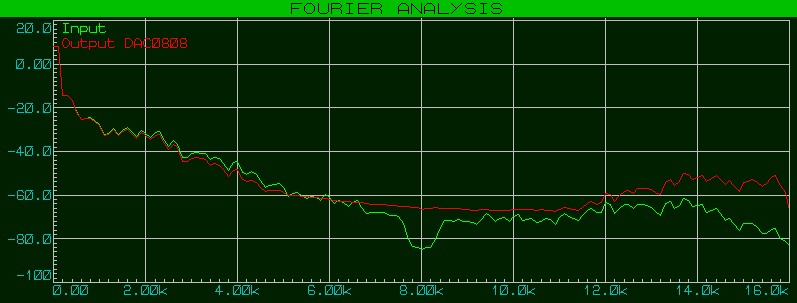
\includegraphics[width=.6\textwidth]{./images/spectrum_mov_avg_2_16k.png}
%             \caption{Analyse fréquentielle}
%         \end{subfigure}
%         \begin{subfigure}[b]{\textwidth}
%             \centering
%             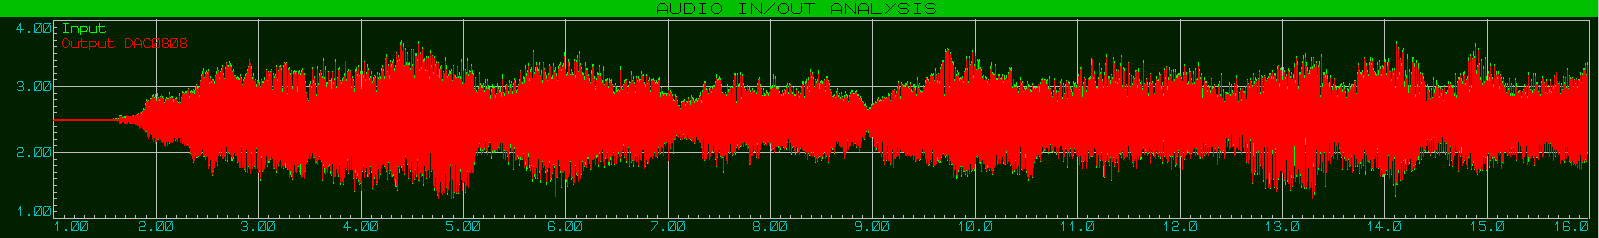
\includegraphics[width=\textwidth]{./images/out_mov_avg_2_16k.png}
%             \caption{Analyse temporelle}
%         \end{subfigure}
%         \caption{Test du filtre par moyenne glissante d'ordre 2 (16kHz)}
%     \end{figure}

%     \subsubsection{Test : filtre d'ordre 4 (16kHz)}
%     \begin{figure}[H]
%         \centering
%         \begin{subfigure}[b]{\textwidth}
%             \centering
%             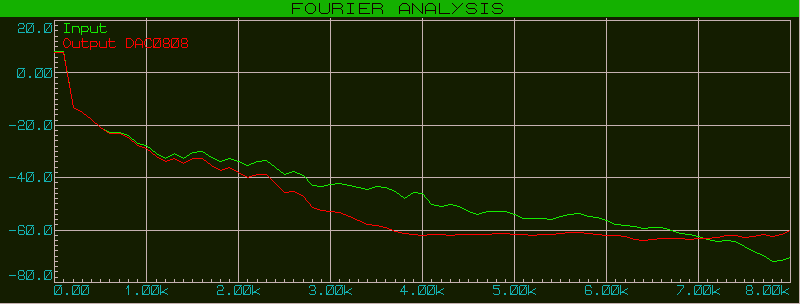
\includegraphics[width=.6\textwidth]{./images/spectrum_mov_avg_4_16k.png}
%             \caption{Analyse fréquentielle}
%         \end{subfigure}
%         \begin{subfigure}[b]{\textwidth}
%             \centering
%             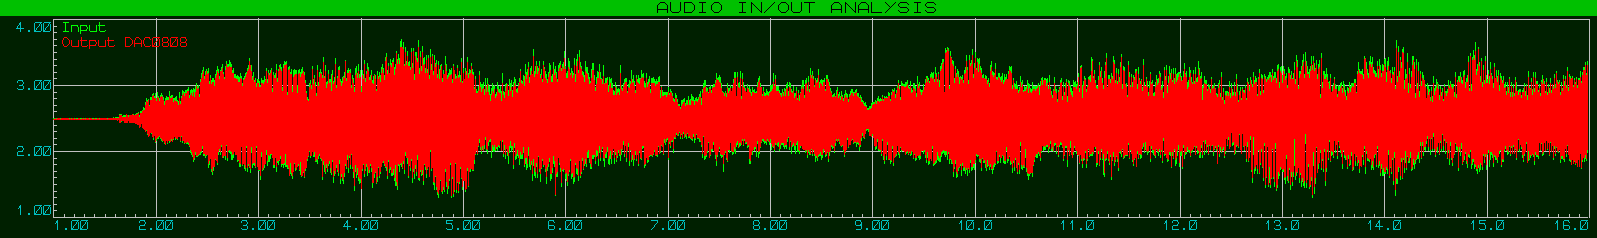
\includegraphics[width=\textwidth]{./images/out_mov_avg_4_16k.png}
%             \caption{Analyse temporelle}
%         \end{subfigure}
%         \caption{Test du filtre par moyenne glissante d'ordre 4 (16kHz)}
%     \end{figure}

%     \subsubsection{Test : filtre d'ordre 8 (16kHz)}
%     \begin{figure}[H]
%         \centering
%         \begin{subfigure}[b]{\textwidth}
%             \centering
%             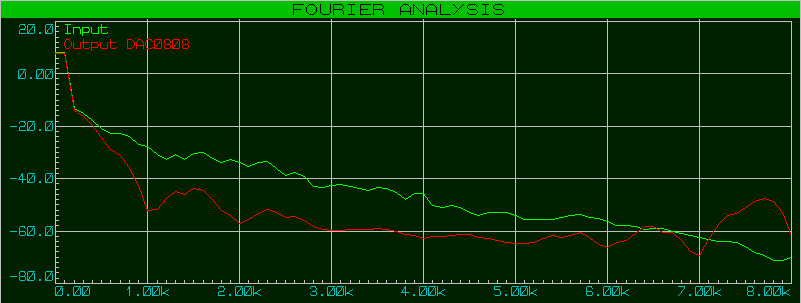
\includegraphics[width=.6\textwidth]{./images/spectrum_mov_avg_8_16k.png}
%             \caption{Analyse fréquentielle}
%         \end{subfigure}
%         \begin{subfigure}[b]{\textwidth}
%             \centering
%             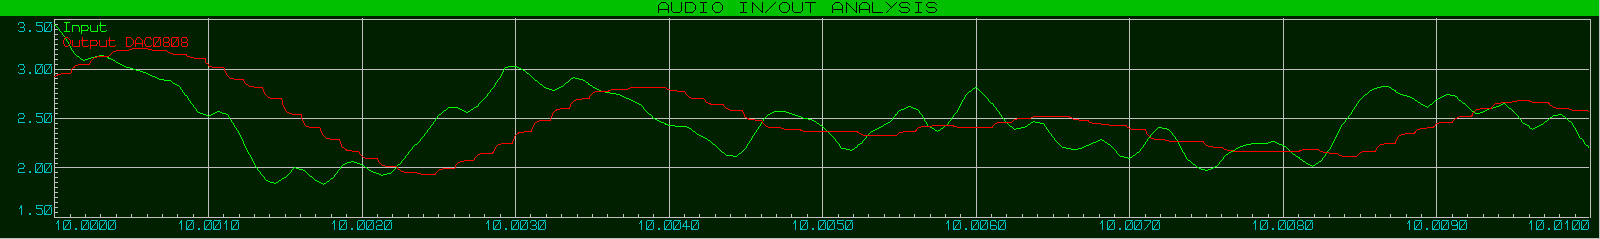
\includegraphics[width=\textwidth]{./images/out_mov_avg_8_16k.png}
%             \caption{Analyse temporelle}
%         \end{subfigure}
%         \caption{Test du filtre par moyenne glissante d'ordre 8 (16kHz)}
%     \end{figure}

%     \subsubsection{Test : filtre d'ordre 2 (8kHz)}
%     \begin{figure}[H]
%         \centering
%         \begin{subfigure}[b]{\textwidth}
%             \centering
%             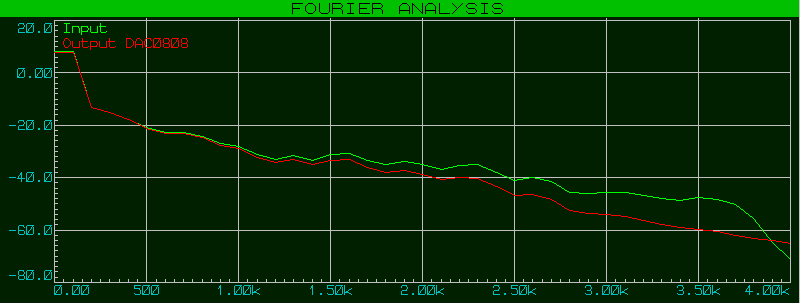
\includegraphics[width=.6\textwidth]{./images/spectrum_mov_avg_2_8k.png}
%             \caption{Analyse fréquentielle}
%         \end{subfigure}
%         \begin{subfigure}[b]{\textwidth}
%             \centering
%             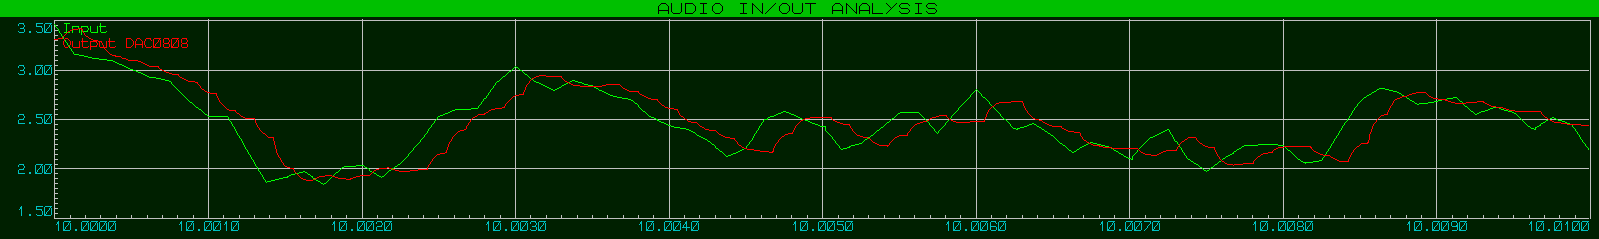
\includegraphics[width=\textwidth]{./images/out_mov_avg_2_8k.png}
%             \caption{Analyse temporelle}
%         \end{subfigure}
%         \caption{Test du filtre par moyenne glissante d'ordre 2 (8kHz)}
%     \end{figure}

%     \subsubsection{Test : filtre d'ordre 4 (8kHz)}
%     \begin{figure}[H]
%         \centering
%         \begin{subfigure}[b]{\textwidth}
%             \centering
%             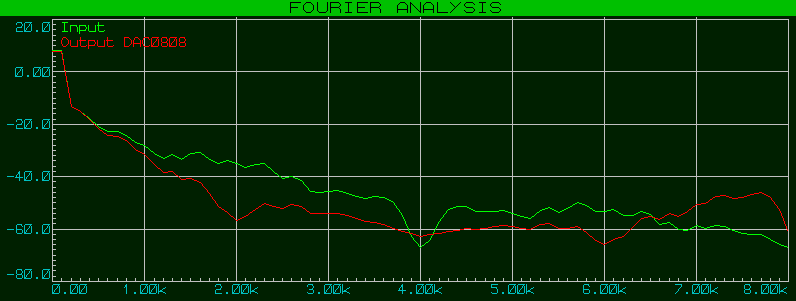
\includegraphics[width=.6\textwidth]{./images/spectrum_mov_avg_4_8k.png}
%             \caption{Analyse fréquentielle}
%         \end{subfigure}
%         \begin{subfigure}[b]{\textwidth}
%             \centering
%             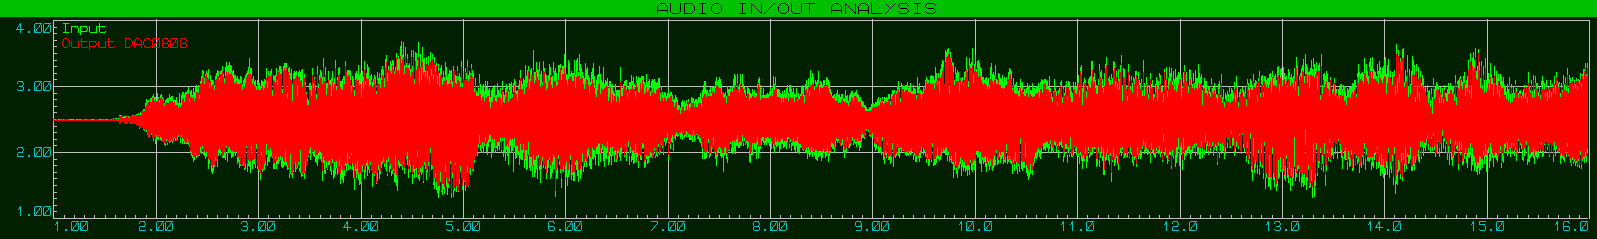
\includegraphics[width=\textwidth]{./images/out_mov_avg_4_8k.png}
%             \caption{Analyse temporelle}
%         \end{subfigure}
%         \caption{Test du filtre par moyenne glissante d'ordre 4 (8kHz)}
%     \end{figure}

%     \subsubsection{Test : filtre d'ordre 8 (8kHz)}
%     \begin{figure}[H]
%         \centering
%         \begin{subfigure}[b]{\textwidth}
%             \centering
%             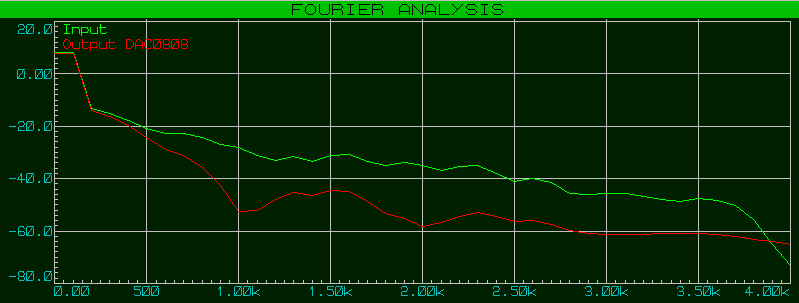
\includegraphics[width=.6\textwidth]{./images/spectrum_mov_avg_8_8k.png}
%             \caption{Analyse fréquentielle}
%         \end{subfigure}
%         \begin{subfigure}[b]{\textwidth}
%             \centering
%             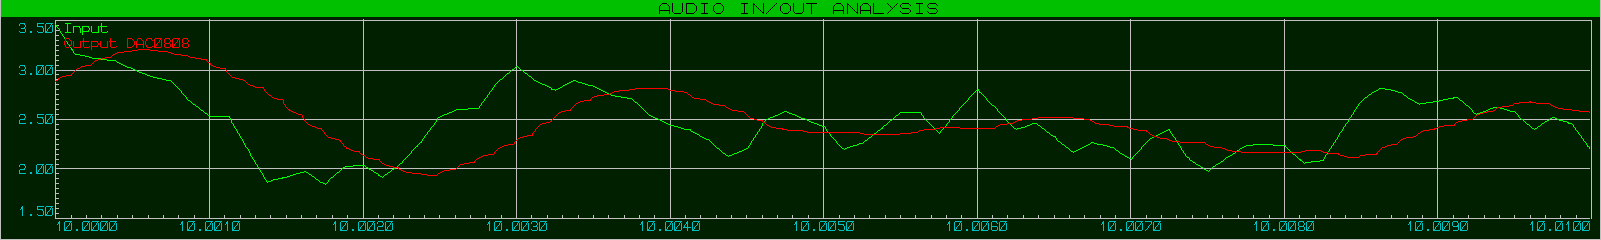
\includegraphics[width=\textwidth]{./images/out_mov_avg_8_8k.png}
%             \caption{Analyse temporelle}
%         \end{subfigure}
%         \caption{Test du filtre par moyenne glissante d'ordre 8 (8kHz)}
%     \end{figure}


%     \subsection{Filtre passe-bas}
%     Le test avec les valeurs limites permet de vérifier que c'est bien un filtre passe-bas : à 0, ne doit rien laisser passer et au max doit tout laisser passer.


%     \subsection{Filtre passe-haut}
%     Comme pour le passe-bas : test avec les valeurs limites.
%     A 0, on laisse bien passer tout le signal.


%     \subsection{Filtre écho}
%     \paragraph{}
%     Le filtre écho a été testé avec les fichiers \emph{angelou\_10s\_delay\_1s\_8k.wav} (pour une fréquence d'échantillonnage de \SI{8}{\kilo\hertz}) et \emph{angelou\_10s\_delay\_1s\_16k.wav} (pour \SI{16}{\kilo\hertz}). Le délai d'une seconde au début du fichier permet de laisser assez de temps au programme pour initialiser le filtre.

%     \subsubsection{Test: 1 écho, durée de 200ms (16kHz)}
%     \paragraph{}
%     Avec une fréquence d'échantillonnage de \SI{16}{\kilo\hertz}, le filtre écho peut fonctionner avec une durée maximale de \SI{200}{\milli\second}. L'audio produit permet d'entendre un léger écho (\emph{test\_echo\_1\_200ms\_16k.wav}).

%     \paragraph{}
%     La comparaison des signaux d'entrée et de sortie de la figure~\ref{fig:echo_16k} met en évidence l'apparition de cet écho (entouré en rouge). Cette figure vérifie également que l'écho apparaît bien \SI{200}{\milli\second} après le signal original: e.g. le deuxième écho mis en évidence sur la figure~\ref{fig:echo_16k_out} démarre à \SI{4.25}{\second}, répercutant le signal original qui démarre à \SI{4.05}{\second} (lignes oranges).

%     \begin{figure}[H]
%         \centering
%         \begin{subfigure}[b]{\textwidth}
%             \centering
%             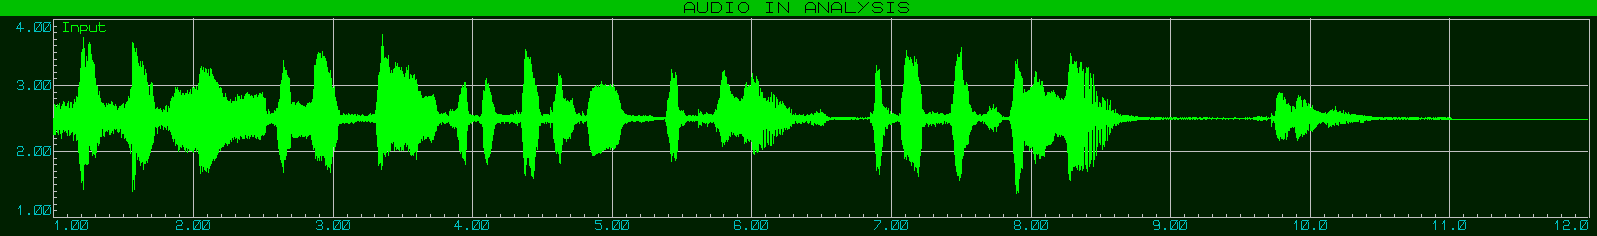
\includegraphics[width=\textwidth]{./images/in_echo_16k.png}
%             \caption{Signal d'entrée}
%         \end{subfigure}
%         \begin{subfigure}[b]{\textwidth}
%             \centering
%             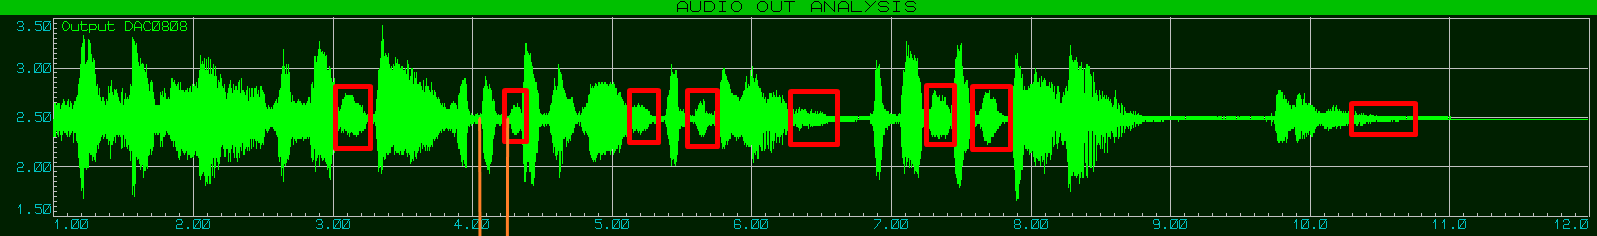
\includegraphics[width=\textwidth]{./images/out_echo_1_200ms_16k.png}
%             \caption{Signal de sortie}
%             \label{fig:echo_16k_out}
%         \end{subfigure}
%         \caption{Test du filtre écho : 1 écho, durée de 200ms (16kHz)}
%         \label{fig:echo_16k}
%     \end{figure}

%     \paragraph{}
%     L'analyse de Fourier des signaux d'entrée et de sortie montre des spectres similaires. À partie de \SI{8}{\kilo\hertz}, le spectre du signal de sortie s'éloigne du spectre du signal d'entrée à cause du bruit de quantification.

%     \begin{figure}[H]
%         \centering
%         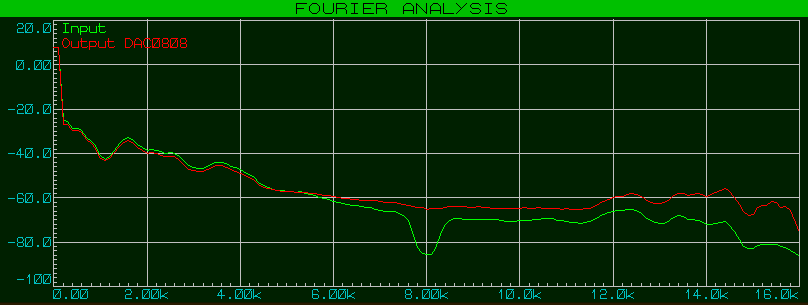
\includegraphics[width=.6\textwidth]{./images/spectrum_echo_1_200ms_16k.png}
%         \caption{Test du filtre écho : spectre de 1 écho, durée de 200ms (16kHz)}
%     \end{figure}

%     \subsubsection{Test: 1 écho, durée de 400ms (8kHz)}
%     \paragraph{}
%     Le filtre écho a également été testé avec un écho de la durée maximale possible pour une fréquence d'échantillonnage de \SI{8}{\kilo\hertz}, i.e. \SI{400}{\milli\second}. L'audio de sortie (\emph{test\_echo\_1\_400ms\_8k.wav}) permet d'entendre clairement cet écho.

%     \paragraph{}
%     La comparaison des signaux d'entrée et de sortie met en évidence l'apparition de cet écho \SI{400}{\milli\second} après le signal original : e.g. le premier écho mis en évidence démarre à \SI{5.12}{\second} et répercute la portion du signal original qui débute à \SI{4.72}{\second} (lignes oranges).

%     \begin{figure}[H]
%         \centering
%         \begin{subfigure}[b]{\textwidth}
%             \centering
%             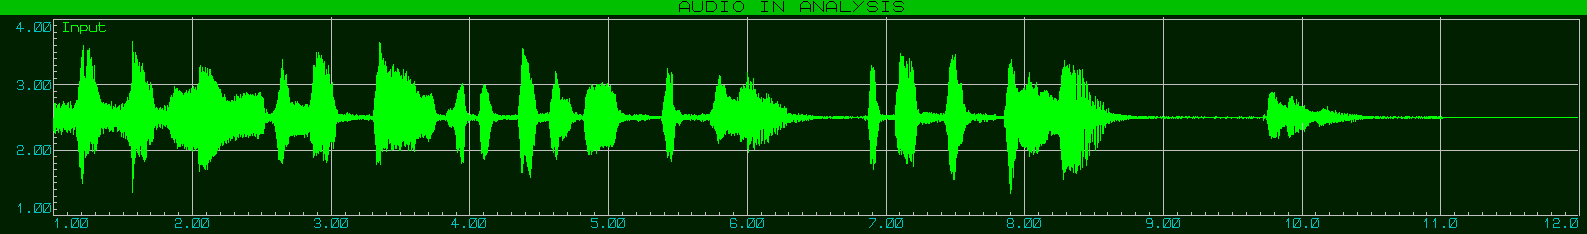
\includegraphics[width=\textwidth]{./images/in_echo_8k.png}
%             \caption{Signal d'entrée}
%         \end{subfigure}
%         \begin{subfigure}[b]{\textwidth}
%             \centering
%             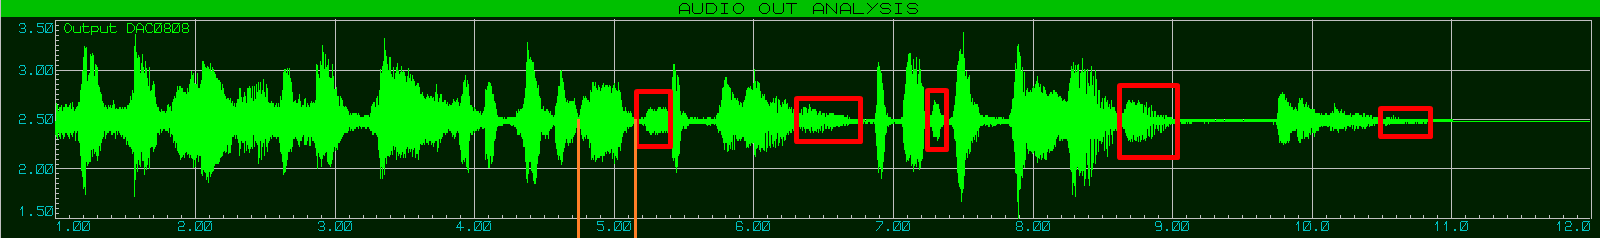
\includegraphics[width=\textwidth]{./images/out_echo_1_400ms_8k.png}
%             \caption{Signal de sortie}
%             \label{fig:echo_8k_out}
%         \end{subfigure}
%         \caption{Test du filtre écho : 1 écho, durée de 400ms (8kHz)}
%     \end{figure}

%     \paragraph{}
%     L'analyse de Fourier est similaire à la précédente : les spectres des signaux d'entrée et de sortie sont identiques jusqu'à \SI{4}{\kilo\hertz} où ils commencent à s'écarter l'un de l'autre à cause du bruit de quantification.

%     \begin{figure}[H]
%         \centering
%         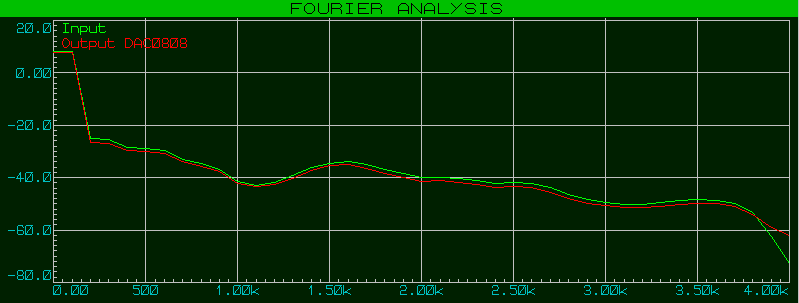
\includegraphics[width=.6\textwidth]{./images/spectrum_echo_1_400ms_8k.png}
%         \caption{Test du filtre écho : spectre de 1 écho, durée de 400ms (8kHz)}
%     \end{figure}

%     \subsubsection{Test: 1 écho, durée de 200ms (8kHz)}
%     \paragraph{}
%     Le filtre écho testé avec un écho d'une durée de \SI{200}{\milli\second} avec une fréquence d'échantillonnage de \SI{8}{\kilo\hertz} donne un résultat similaire au premier test. L'audio de sortie \emph{test\_echo\_1\_200ms\_8k.wav} permet d'entendre le même écho malgré la qualité d'audio moindre. Le signal de sortie est similaire : les échos apparaissent aux mêmes endroits, décalés de \SI{200}{\milli\second} par rapport au signal original.
%     \begin{figure}[H]
%         \centering
%         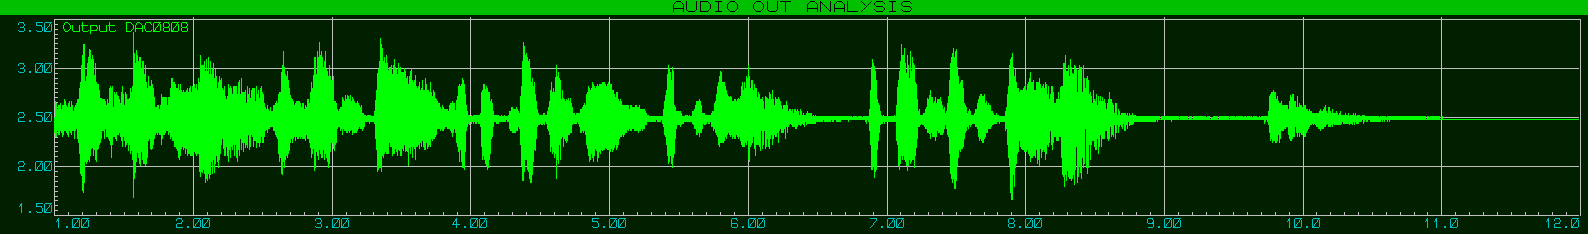
\includegraphics[width=\textwidth]{./images/out_echo_1_200ms_8k.png}
%         \caption{Test du filtre écho : output de 1 écho, durée de 200ms (8kHz)}
%     \end{figure}

%     \subsubsection{Test: 1 écho, durée de 100ms (8kHz)}
%     \paragraph{}
%     Avec une durée de \SI{100}{\milli\second}, l'écho n'est presque plus perceptible (\emph{test\_echo\_1\_100ms\_8k.wav}). Les échos générés sont bien visibles sur l'analyse du signal de sortie, décalés de \SI{100}{\milli\second} par rapport au signal original.
%     \begin{figure}[H]
%         \centering
%         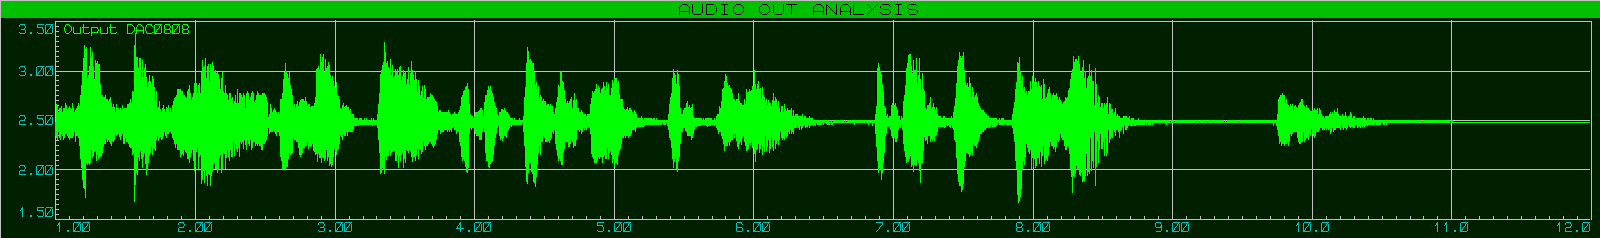
\includegraphics[width=\textwidth]{./images/out_echo_1_100ms_8k.png}
%         \caption{Test du filtre écho : output de 1 écho, durée de 100ms (8kHz)}
%     \end{figure}

%     \subsubsection{Test: 2 échos, durée de 400ms (8kHz)}
%     \paragraph{}
%     Les échos multiples ont été testés avec une fréquence d'échantillonnage de \SI{8}{\kilo\hertz} puisqu'elle autorise une durée deux fois plus grande qu'à \SI{16}{\kilo\hertz}. La durée est réglée au maximum (\SI{400}{\milli\second}) pour pouvoir distinguer au mieux le signal original et ses échos.

%     \paragraph{}
%     Comme avec un seul écho, le signal original apparaît affaibli. Les échos sont moins marqués mais apparaissent bien et surtout sont bien distinguables à l'écoute (\emph{test\_echo\_2\_8k.wav}).
%     \begin{figure}[H]
%         \centering
%         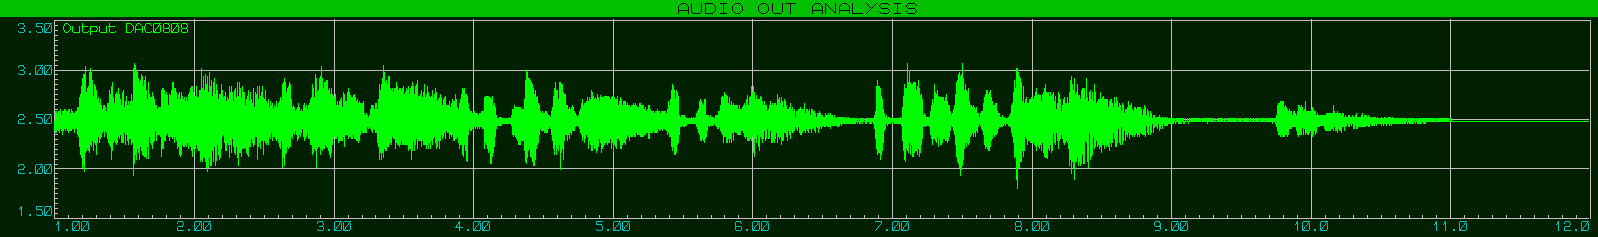
\includegraphics[width=\textwidth]{./images/out_echo_2_8k.png}
%         \caption{Test du filtre écho : output de 2 échos, durée de 400ms (8kHz)}
%     \end{figure}

%     \subsubsection{Test: 3 échos, durée de 400ms (8kHz)}
%     \paragraph{}
%     Avec trois échos, le signal original est encore plus atténué et les échos sont plus fondus. Ils sont maintenant difficilement distinguables à l'écoute (\emph{test\_echo\_3\_8k.wav}).

%     \begin{figure}[H]
%         \centering
%         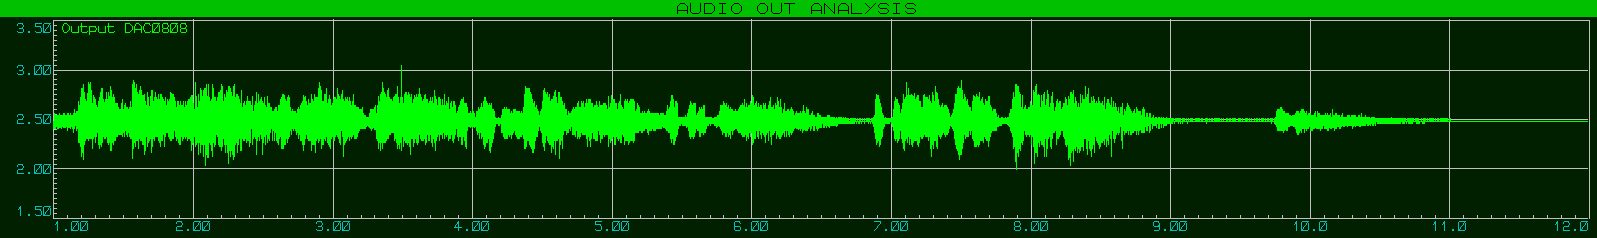
\includegraphics[width=\textwidth]{./images/out_echo_3_8k.png}
%         \caption{Test du filtre écho : output de 3 échos, durée de 400ms (8kHz)}
%     \end{figure}


%     \newpage
%     \section{Difficultés rencontrées}
%     % Le calcul des mises à échelle pour s'assurer qu'il n'y a pas de dépassement de valeurs.

%     % concevoir un programme qui fonctionne bien en simulation

%     % proposer à la fois un menu assez riche et économiser l'espace pour le réserver pour les buffers: il n'y avait pas durée d'écho minimale précisée donc ça va mais j'aurais clairement pu faire mieux (aller jusqu'à 450 ms pour du 8k)

%     % \section{Configuration}





%     % 1/03 interruptions prioritisées
%     Possible amélioration mais complique beaucoup la programmation. En plus, en 16kHz, on est vraiment à la limite des possibilités du processeur -> beaucoup d'interruptions en haute priorité -> les entrées et sorties risquent d'être extrêmement


% parler aussi de la taille max des buffers en fonction de la mémoire du PIC



\end{document}